%------------------------------------------------------------------------------
%	MOTIVATION
%------------------------------------------------------------------------------


\subsection{Motivation}

An ever-important issue regarding civil infrastructure or in general engineering systems is their deterioration over time. Deterioration is a serious concern since it often leads to the reduction of structural capacity as well as the reliability and service life of a system. Many instances showcase the importance of structural degradation, with structures located in coastal and marine environments being the most common cases, as well as structures subjected to cyclic loading, hence fatigue. Typical examples of deteriorating systems constitute bridges \cite{stewart1998time}, \cite{akgul2004lifetime}, \cite{val1998effect}, offshore platforms \cite{moan2005reliability}, \cite{lotsberg2016probabilistic}, \cite{wirsching1980fatigue}, and wind turbines \cite{schaumann2011special}, \cite{dong2012fatigue}, \cite{yeter2015fatigue}. In particular, in cases of structural steel, it is most likely that galvanic corrosion will occur due to the atmospheric exposure in a marine environment, whereas the deterioration of reinforced concrete elements takes place in the form of corrosion of the reinforcement and/or spalling of the concrete. Lastly, fatigue can also lead to significant degradation of the structure, being responsible for the formation and the propagation of cracks.\\

However, these degradation processes are highly stochastic, and their prediction often requires a probabilistic analysis, having first expressed quantitatively the uncertainties, which are involved in these physical procedures. Therefore, the maintenance of a deteriorating system constitutes a complex sequential decision-making problem under uncertainty, for which it is often intractable to find closed-form solutions concerning the optimal actions that accomplish a plethora of life-cycle objectives. Additionally, the existence of multiple components, their interaction, and their ability to mitigate one another's failure, contribute to the enhancement of the uncertainty and the difficulty to define an optimal sequence of actions that will fulfill long-term goals.\\

To define the actual degradation of a system, a common practice is to employ new information derived from monitoring devices, to update the prior knowledge of a system's parameters. This non-destructive damage assessment, i.e. incorporating observations based on \gls{SHM}, can reflect the actual deterioration, leading to a decreased variability of the system's current condition and structural capacity, hence to more realistic and accurate modeling of it, allowing the decision-maker to proceed with more informed and rational decisions. The majority of these updating techniques rely on Bayesian principles and the notion of \gls{BMU}.\\

As far as the optimal maintenance policy is concerned, due to the significant amount of deterioration states, possible maintenance actions, and the decision steps under consideration, analytical solutions for determining the wanted optimal sequence of actions are more often than not computationally heavy. The so-called curse of dimensionality has been alleviated with the use of \gls{RL} techniques, which were able to provide approximate solutions for optimal maintenance policies for engineering systems. Even further progress was achieved when, in 2014, DeepMind patented an application of \gls{RL} techniques to \gls{DL}, with the scope of playing Atari games better than human experts \cite{mnih2013playing}. This new approach, namely \acrfull{DRL}, overcame the limitations that traditional \gls{RL} had, and was proved to be a promising tool for finding near-optimal control policies.


%------------------------------------------------------------------------------
%	PROBLEM STATEMENT
%------------------------------------------------------------------------------


\subsection{Problem Statement} \label{ProbState}

The scope of this thesis is the development of an integrated framework that will combine \gls{DRL} techniques with Bayesian Inference, with the former tackling the sequential decision optimization, while the latter one would deal with the accurate modeling of the stochastic deterioration process. The ultimate goal of this tool is to determine the optimal sequence of maintenance decisions that result to the minimum cost throughout the service life of an engineering system. To elaborate further on the interaction between the various elements that will be used in this framework, response quantities of the system, that are contaminated with noise, will be fed into an \gls{OMA} procedure, in order to obtain modal characteristics (also including some uncertainty, through additional noise). Furthermore, the transition of the system to its new state will be described by a stochastic deterioration model, which will be constantly more accurate by incorporating observations during each decision step. A generic schematic representation of the aforementioned problem is depicted in Figure \ref{genProb}.

\begin{figure}[H]
    \centering
	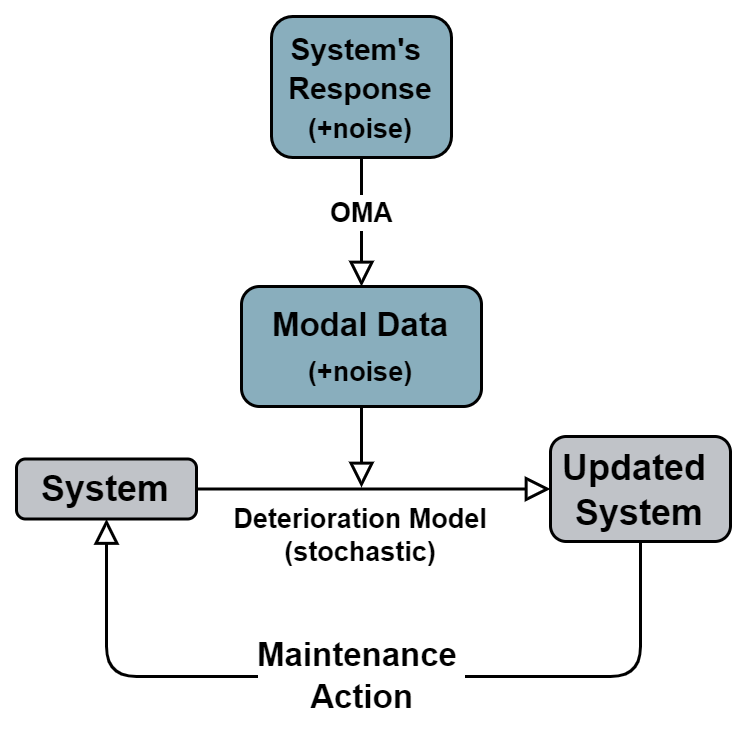
\includegraphics[width=0.5\linewidth]{Figures/basicFlow.png}
	\caption{Problem Statement - General Framework}
	\label{genProb}
\end{figure}

\newpage

The necessary \textbf{inputs} are:

\begin{itemize}
    \item Initial (prior) distribution for system parameters (e.g. stiffness, mass, deterioration parameters,~etc)
    \item Stochastic deterioration model over time
    \item Possible actions (e.g. do nothing, repair, replace, etc)
    \item Cost definition (e.g. action costs, risk of failure)
    \item Noise interfering in observations' monitoring
    \item Time window of interest
\end{itemize}

The \textbf{ouput} of the proposed framework will be the optimal sequence of actions, that minimize the cost function, over the system's service~life.\\

It should be mentioned, that such a coupling of these two core concepts, namely \gls{DRL} and \gls{BMU}, has not been done yet in the existing research (as will be thoroughly presented in Chapter \ref{LitReview}), especially in the field of infrastructure maintenance, a fact that highlights the innovation of the proposed framework. Nevertheless, owing to the limited assumptions and simplifications that will be considered for the sake of accuracy, it is likely that considerable challenges and obstacles may be posed regarding the computational costs.


%------------------------------------------------------------------------------
%	RESEARCH QUESTION
%------------------------------------------------------------------------------


\subsection{Research Question} \label{researchQ}

The research question can be formulated as follows:

\begin{quote}
    \emph{“How to develop an integrated framework that will efficiently couple \acrfull{DRL} algorithms and \acrfull{BMU} when it comes to structural systems' life cycle optimization, using vibration data/observations? ”}
\end{quote}

In order to efficiently reach the answer to the main research question, it is further broken down into the following sub-questions:
\begin{itemize}
    \item How can this framework be applied in a simplified yet representative case (toy problem)?
    \item Having produced sound results for the simple case, which \gls{DRL} algorithm performs better?
    \item Due to the significant computational cost of \gls{BMU}, how can it be integrated in a more time-efficient way?
    \item Can this framework be scaled up to more complicated cases? (e.g. bigger action spaces, complex multi-component structures, etc)
\end{itemize}

\newpage

%------------------------------------------------------------------------------
%	RESEARCH METHODOLOGY
%------------------------------------------------------------------------------

\subsection{Research Methodology}

The research of the current problem can be structured in four main sections, as illustrated also in Figure \ref{researchMeth}. The research framework constitutes the first part, including the motivation, the definition of the problem statement and a clear formulation of the research question. The second part focuses on the literature review, according to which the research objectives and questions might be refined. Having laid the theoretical foundation, and built an informed picture of the existing research, the tool development follows, as well as the formulation of the applications on which the proposed tool will be tested. In the current project, two problems of different complexity will be addressed, with the minor one acting also as a validation and verification test for the proposed framework. The culmination of the aforementioned steps will be the evaluation of the results, accompanied by the corresponding discussions and considerations about future developments, based on the showcased strengths and weaknesses of the tool.


\begin{figure}[H]
    \centering
	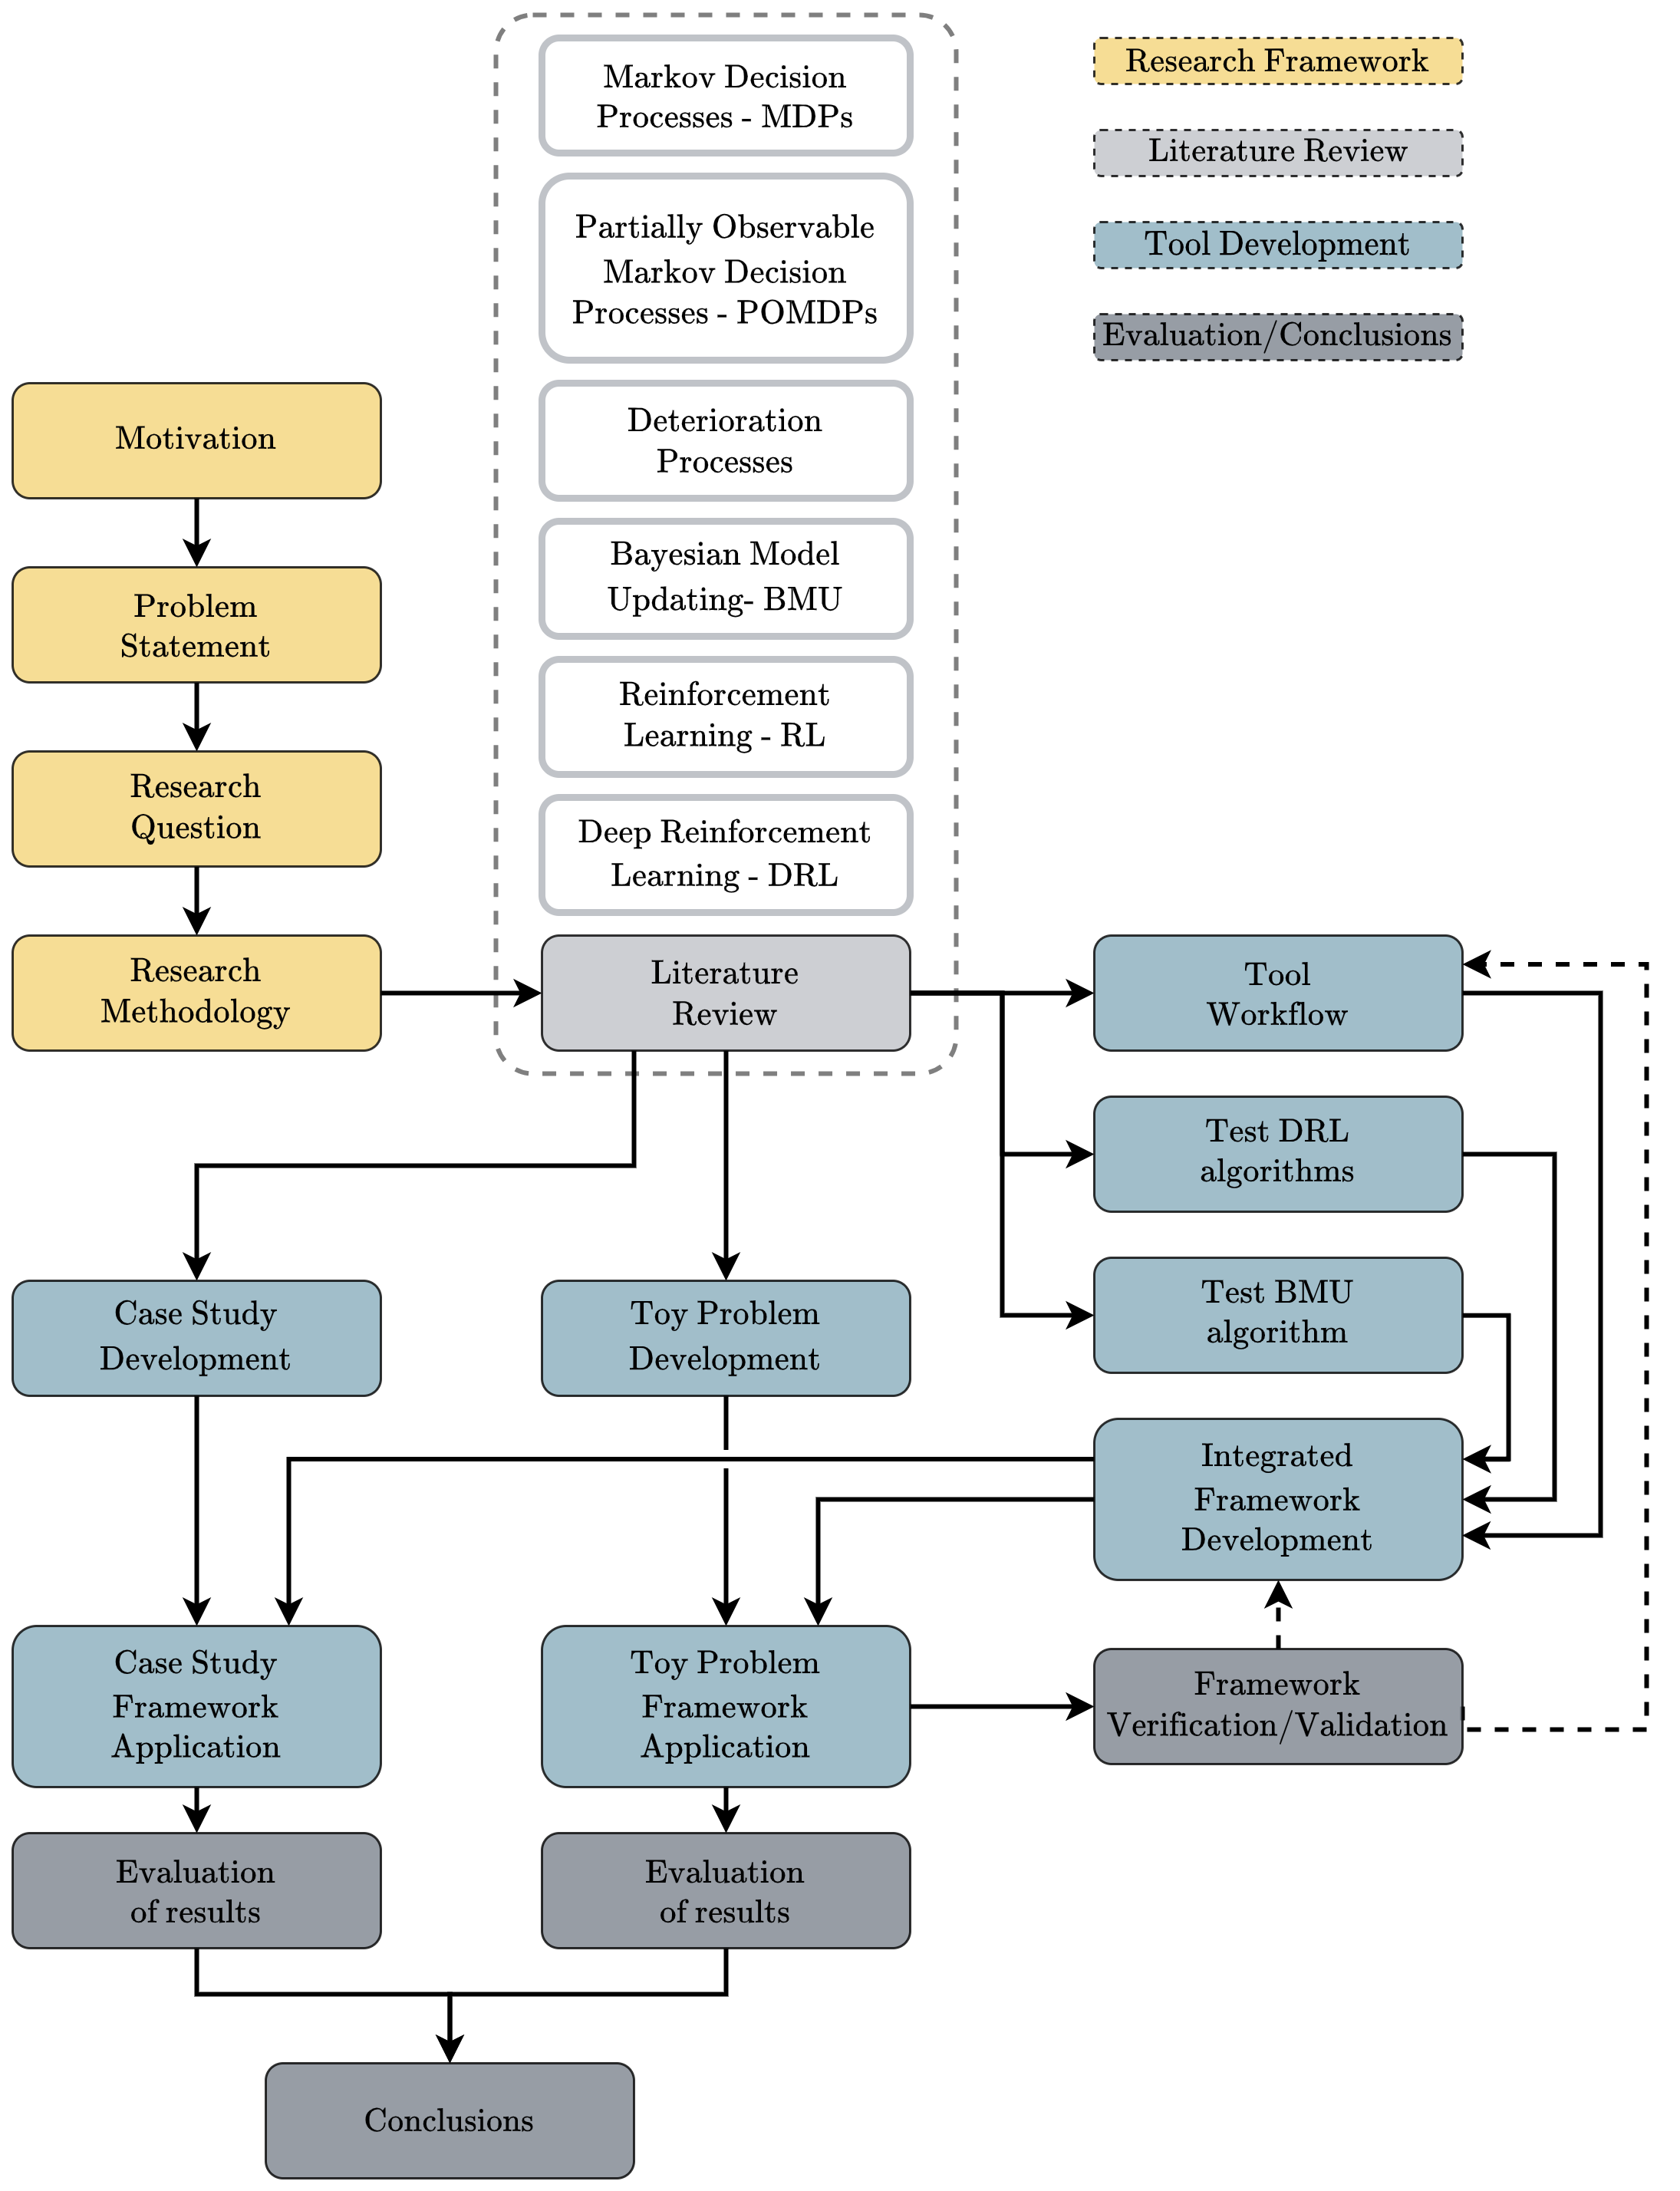
\includegraphics[width=0.97\linewidth]{Figures/researchMethodology.png}
	\caption{Research Methodology flowchart}
	\label{researchMeth}
\end{figure}

The sheer amount of mathematical operations and algorithms that are required for the current project, will be handled with \verb|Python| programming language. A summary of the core libraries/packages that will be needed, is displayed in Figure \ref{packs}.

\begin{figure}[H]
    \centering
	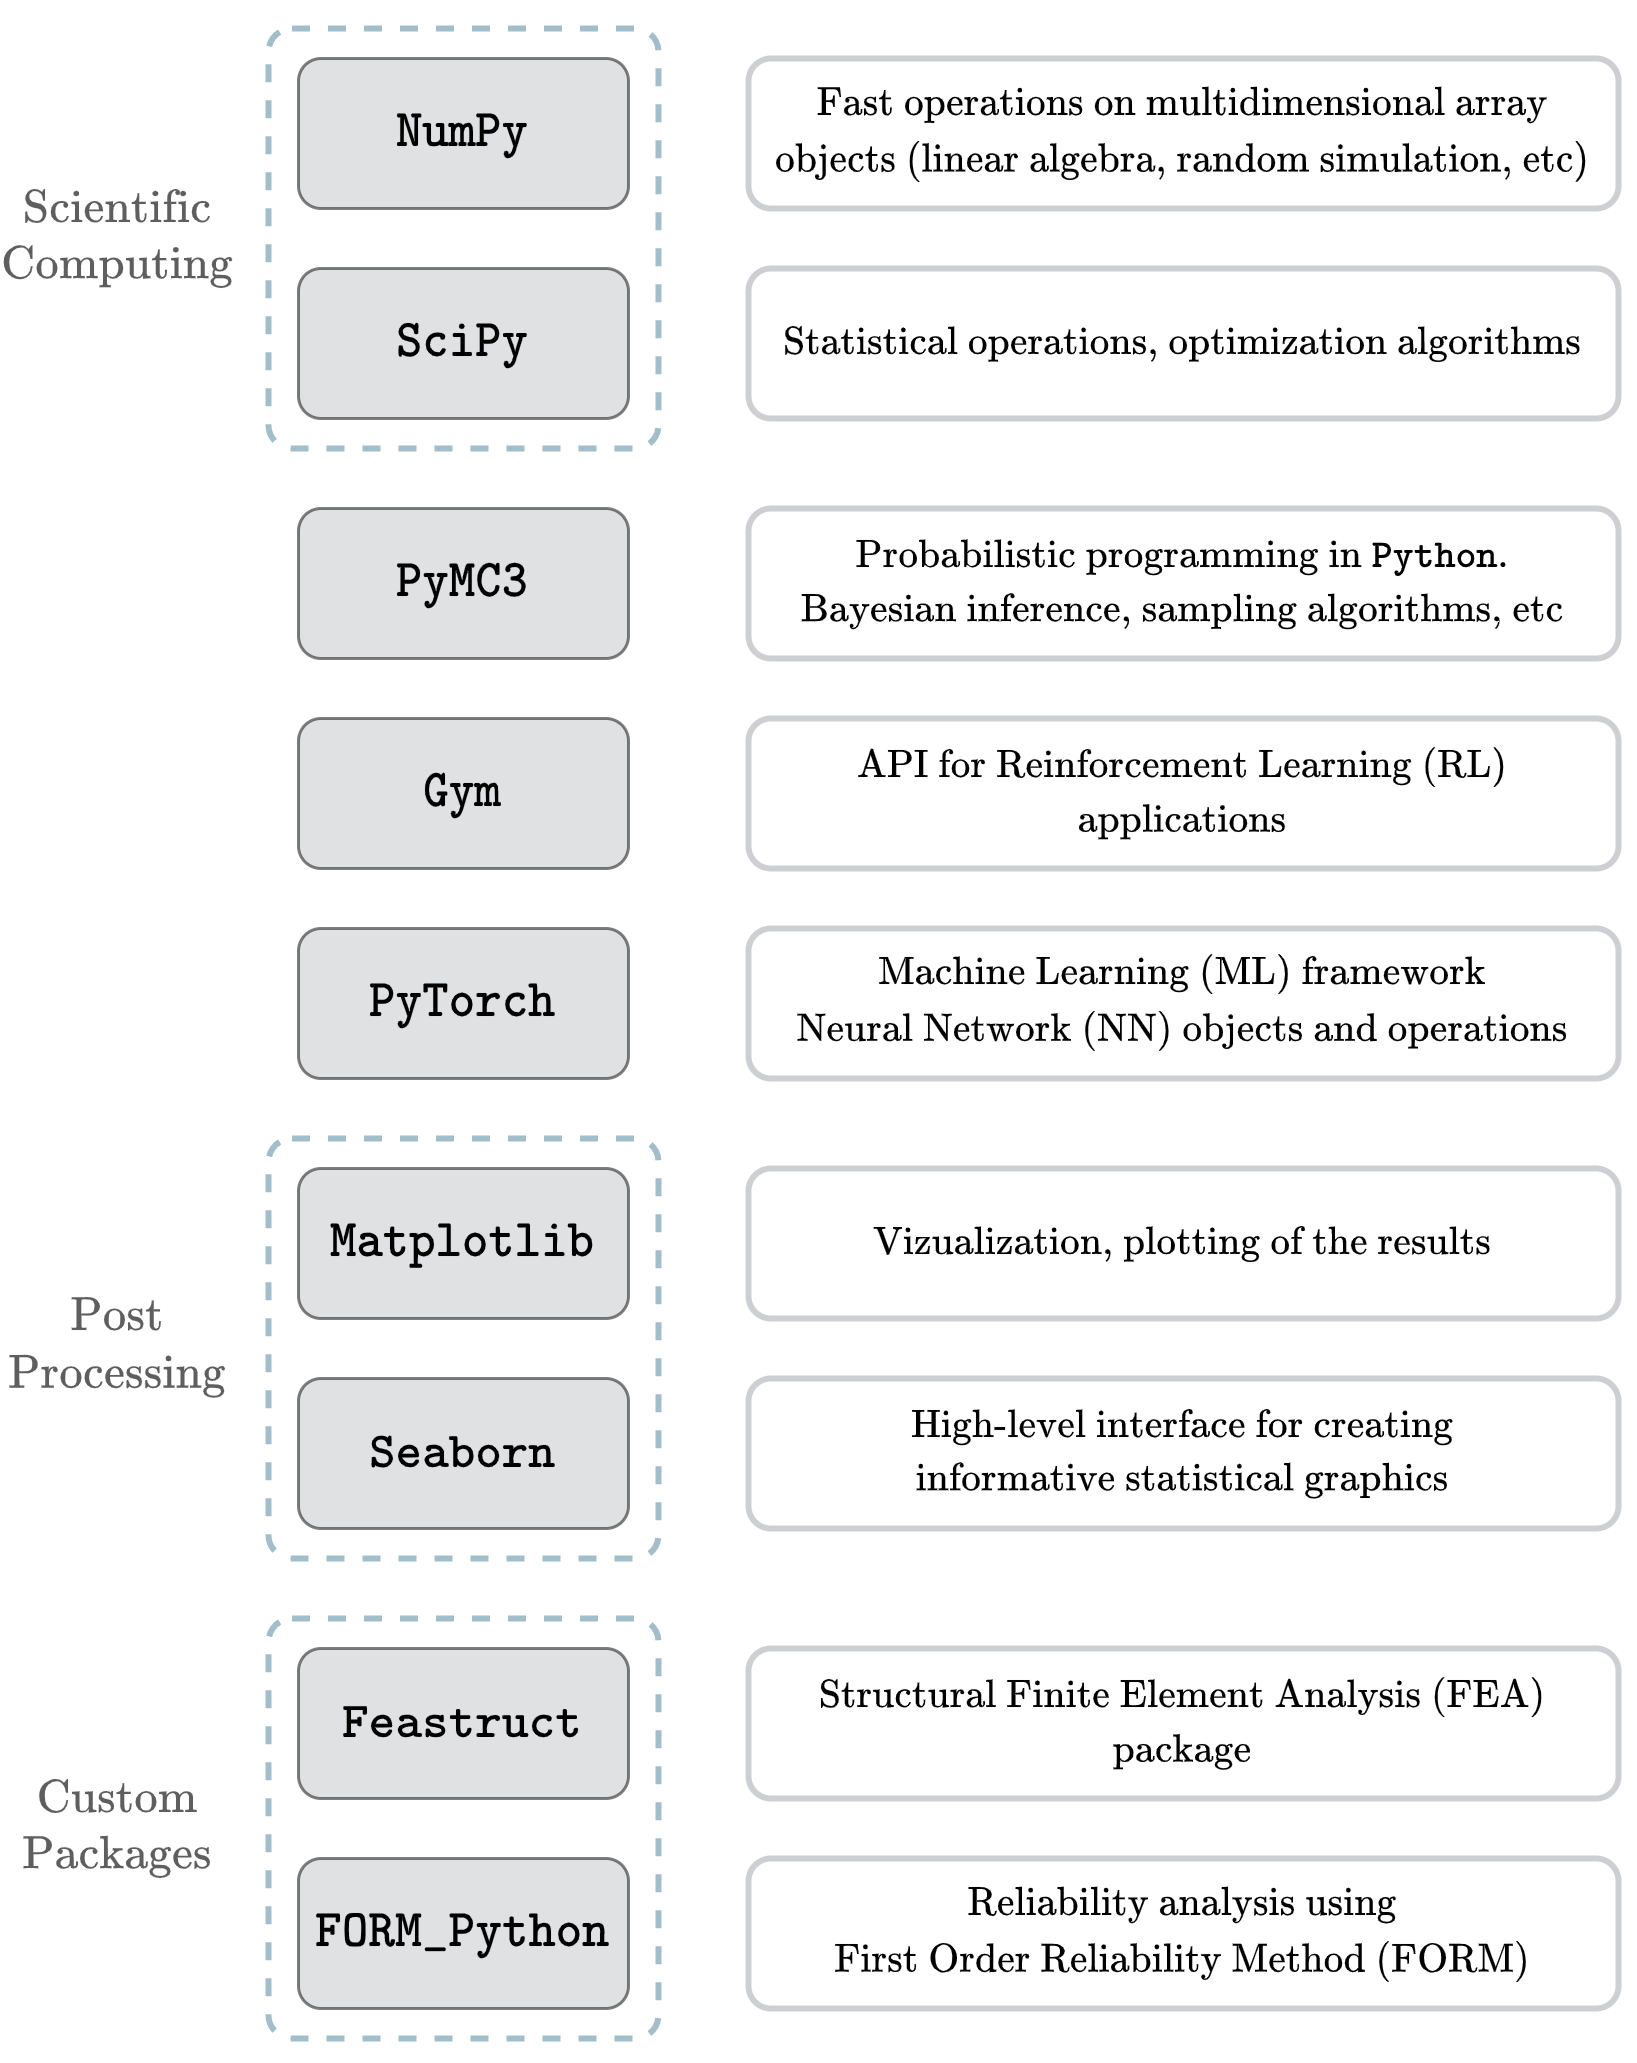
\includegraphics[width=0.85\linewidth]{Figures/packages.png}
	\cprotect\caption{Core \verb|Python| dependencies\footnotemark}
	\label{packs}
\end{figure}

\footnotetext{Apart from the Python libraries, that are widely used for similar projects, there will be use of other, custom ones, that were available open-source, online \cite{robbie2018}, \cite{formTUM2020}}

%------------------------------------------------------------------------------
%	THESIS STRUCTURE
%------------------------------------------------------------------------------


\subsection{Thesis Structure} 

In concluding this introductory chapter, the content of the following ones will be briefly described, further elaborating along with the research methodology flowchart (Figure \ref{researchMeth}) on the structure of the whole thesis. In the coming chapter, the literature review is introduced (Chapter \ref{LitReview}), followed by the description of the methodology of the proposed framework in a generic fashion (Chapter \ref{workflow}). A simple toy problem is presented in the following chapter, where the aforementioned tool is applied (Chapter \ref{toy}). Then, the developed framework is further applied to a more complicated and realistic case study (Chapter \ref{caseStud}), leading to the final chapter, where the main conclusions are drawn, along with a reflection on the advantages and disadvantages of the proposed method, as well as topics for further discussion and future work (Chapter \ref{discConcl}).